\documentclass{beamer}
\mode<presentation>
\usepackage{amsmath}
\usepackage{amssymb}
%\usepackage{advdate}
\usepackage{adjustbox}
\usepackage{subcaption}
\usepackage{enumitem}
\usepackage{multicol}
\usepackage{listings}
\usepackage{url}
\def\UrlBreaks{\do\/\do-}
\usetheme{Madrid}
\usecolortheme{beaver}
\setbeamertemplate{footline}
{
  \leavevmode%
  \hbox{%
  \begin{beamercolorbox}[wd=\paperwidth,ht=2.25ex,dp=1ex,right]{author in head/foot}%
    \insertframenumber{} / \inserttotalframenumber\hspace*{2ex} 
  \end{beamercolorbox}}%
  \vskip0pt%
}
\setbeamertemplate{navigation symbols}{}

\providecommand{\nCr}[2]{\,^{#1}C_{#2}} % nCr
\providecommand{\nPr}[2]{\,^{#1}P_{#2}} % nPr
\providecommand{\mbf}{\mathbf}
\providecommand{\pr}[1]{\ensuremath{\Pr\left(#1\right)}}
\providecommand{\qfunc}[1]{\ensuremath{Q\left(#1\right)}}
\providecommand{\sbrak}[1]{\ensuremath{{}\left[#1\right]}}
\providecommand{\lsbrak}[1]{\ensuremath{{}\left[#1\right.}}
\providecommand{\rsbrak}[1]{\ensuremath{{}\left.#1\right]}}
\providecommand{\brak}[1]{\ensuremath{\left(#1\right)}}
\providecommand{\lbrak}[1]{\ensuremath{\left(#1\right.}}
\providecommand{\rbrak}[1]{\ensuremath{\left.#1\right)}}
\providecommand{\cbrak}[1]{\ensuremath{\left\{#1\right\}}}
\providecommand{\lcbrak}[1]{\ensuremath{\left\{#1\right.}}
\providecommand{\rcbrak}[1]{\ensuremath{\left.#1\right\}}}
\theoremstyle{remark}
\newtheorem{rem}{Remark}
\newcommand{\sgn}{\mathop{\mathrm{sgn}}}
\providecommand{\abs}[1]{\left\vert#1\right\vert}
\providecommand{\res}[1]{\Res\displaylimits_{#1}} 
\providecommand{\norm}[1]{\lVert#1\rVert}
\providecommand{\mtx}[1]{\mathbf{#1}}
\providecommand{\mean}[1]{E\left[ #1 \right]}
\providecommand{\fourier}{\overset{\mathcal{F}}{ \rightleftharpoons}}
%\providecommand{\hilbert}{\overset{\mathcal{H}}{ \rightleftharpoons}}
\providecommand{\system}{\overset{\mathcal{H}}{ \longleftrightarrow}}
	%\newcommand{\solution}[2]{\textbf{Solution:}{#1}}
%\newcommand{\solution}{\noindent \textbf{Solution: }}
\providecommand{\dec}[2]{\ensuremath{\overset{#1}{\underset{#2}{\gtrless}}}}
\newcommand{\myvec}[1]{\ensuremath{\begin{pmatrix}#1\end{pmatrix}}}
\let\vec\mathbf

\lstset{
%language=C,
frame=single, 
breaklines=true,
columns=fullflexible
}

\numberwithin{equation}{section}

\title{Recurent Neural Network}
\author{Tadipatri Uday Kiran Reddy\\EE19BTECH11038 \\ Dept. of Electrical Engg.,\\IIT Hyderabad.}

%\date{\today} 
\logo{
\includegraphics[height=1.5cm]{./figs/logo.jpg}}
\begin{document}

\begin{frame}
\titlepage
\end{frame}

\section*{Outline}
\begin{frame}
\tableofcontents
\end{frame}
%\subsection{Literature}
\section{Zero Padding}
\begin{frame}
\frametitle{Zero Padding}
This is a technique to incrase no of samples of a given audio sample
\begin{description}[font=$\bullet$~\normalfont\scshape\color{red!50!black}]
\item [] Declare an empty array of fixed length which is same length for training the data
\item [] Add the data of the audio sample in the array
\item [] Do this in a circular shift way untill desired no of samples are required
\end{description}

\end{frame}

%\subsection{Literature}
\section{Feature Extraction}
\begin{frame}
\frametitle{MFCC - Mel Frequency Cepstral Coefficient}
%\framesubtitle{Literature}
 MFCC takes into account human perception for sensitivity at appropriate frequencies by converting the conventional frequency to Mel Scale.\\
 \begin{equation*}
     Mel(f) = 1125\ln({1 + \frac{f}{700}})
 \end{equation*}
 In our case, it returns a matrix of (49X39) i.e,49 time steps and each with 39 features.
\end{frame}

\section{Recurent Neural Networks}
\begin{frame}
\frametitle{Motivation for Recurent Neural Network}
The main advantage of the neural neural network over others is its memory for processing Temporal signals\\
Where as in Feedforward Neural Networks such as MLPN's at time t for a input {$x$(f)}_{t\geq0}\\ output would be {f(w,x(t))}_{t\geq0},{\textbf{without regard to the previous history}}.

\end{frame}

\begin{frame}
\frametitle{Recurent Neural Networks}
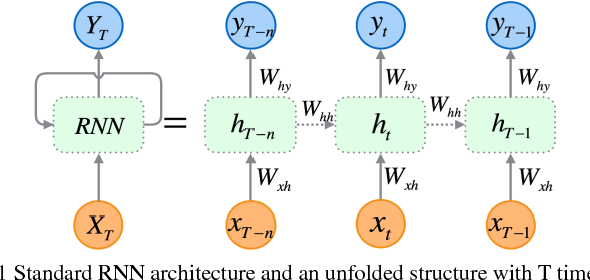
\includegraphics[width=0.5\columnwidth]{./figs/RNN.png}\\
Here $h_t$ is the hidden state at time step t\\
\begin{equation*}
    {h_t}=f({x_t}{W_{xh}} + {W_{hh}}{h_{t-1}})
\end{equation*}\\
where f is a non-linear function\\
For intial hidden state is initialised with all zeros
\end{frame}
\begin{frame}{Back Propagation}
    \begin{equation*}
        {o_t} = softmax({V_{st}})\\
        E(y_t,\hat{y_t}) = -{y_t}\log{\hat{y_t}}\\
        E(y,\hat{y}) = \sum_{n =1}^{T} E(y_t,\hat{y_t})\\
    \end{equation*}
    Now we have learn the data with the gradient $\frac{\partial E}{\partial y}$ back along the chain\\
    Also known as Back Propagation(stochastic descent method).\\
    But the disadvantage is that the gradient vanishes along the chain.
\end{frame}
\section{LSTM}
\begin{frame}{LSTM - Long short Term Memory }
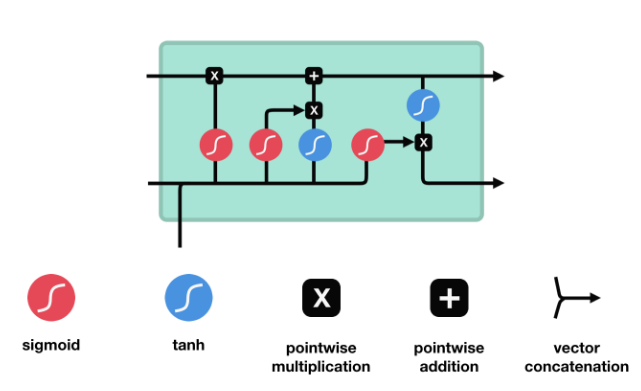
\includegraphics[width=0.8\columnwidth]{./figs/LSTM.png}\\
These operations are used to allow the LSTM to keep or forget information.\\
It has forget gate which decides whether to hold the information or not.\\
This ensures that learning rate does not decrease down the chain.
\end{frame}
\end{document}
